\chapter{Исследовательская часть}
\section{Характеристики устройства}

Исследования проводились на машине со следующими характеристиками:
\begin{itemize}[label=---]
	\item процессор Intel(R) Core(TM) i5-10210U, тактовая частота 1.60 ГГц;
	\item оперативная память: 16 ГБ;
	\item операционная система: Ubuntu 22.04.4 LTS.
\end{itemize}

\section{Замер числа операций сравнений}

Длинна массива по варианту составляет 1041 элемент. Соответственно, было произведено 1042 запуска: для каждого элемента и один для элемента, которого в массиве нет.

Далее приведены графики, иллюстрирующие зависимость количества сравнений от индекса вхождения элемента (для элемента, которого нет в массиве, индекс принимается равным -1). На рисунке~\ref{fig:lin_plot} представлен график для линейного поиска. На рисунке~\ref{fig:bin_plot} для бинарного соответственно.
\begin{figure}[H]
	\centering
	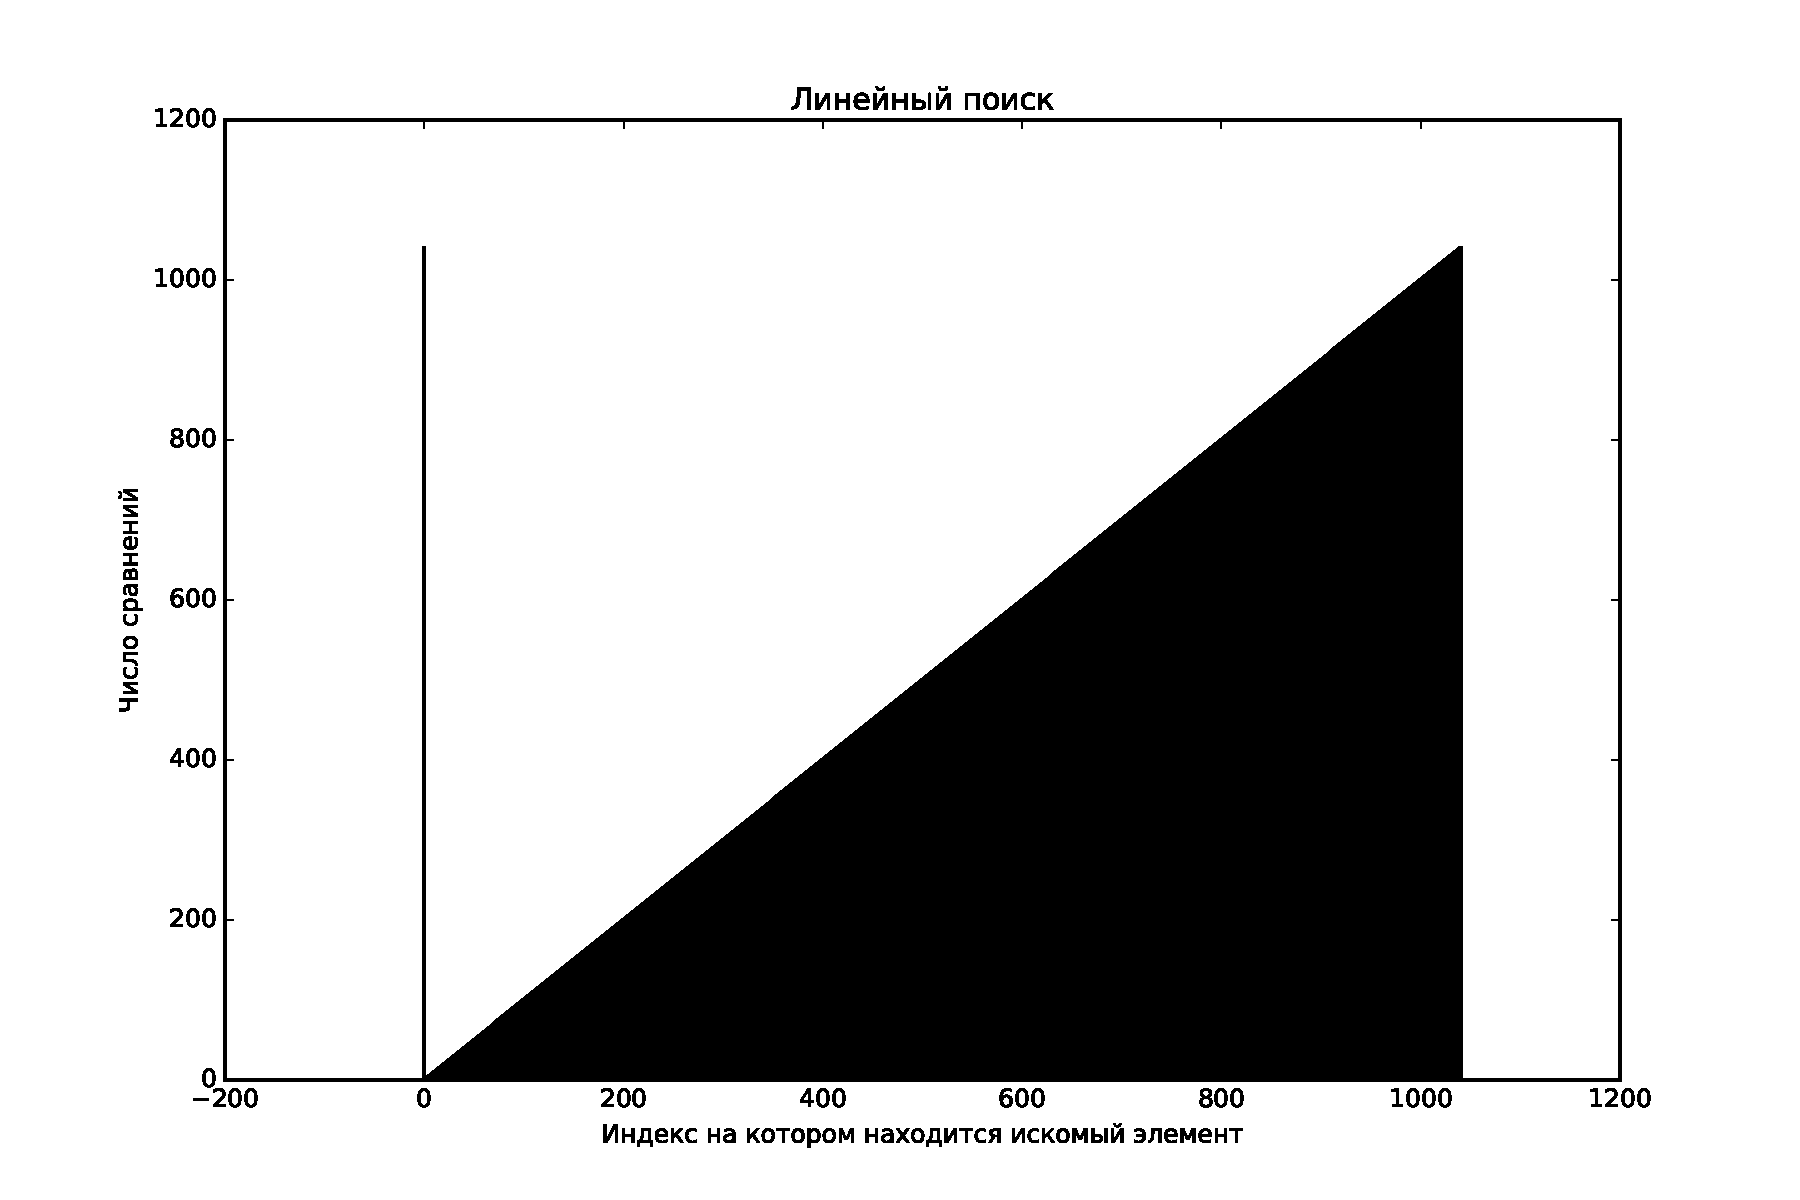
\includegraphics[width=\textwidth]{linear.pdf}
	\caption{График зависимости числа сравнений от индекса элемента для линейного поиска}
	\label{fig:lin_plot}
\end{figure}
\begin{figure}[H]
	\centering
	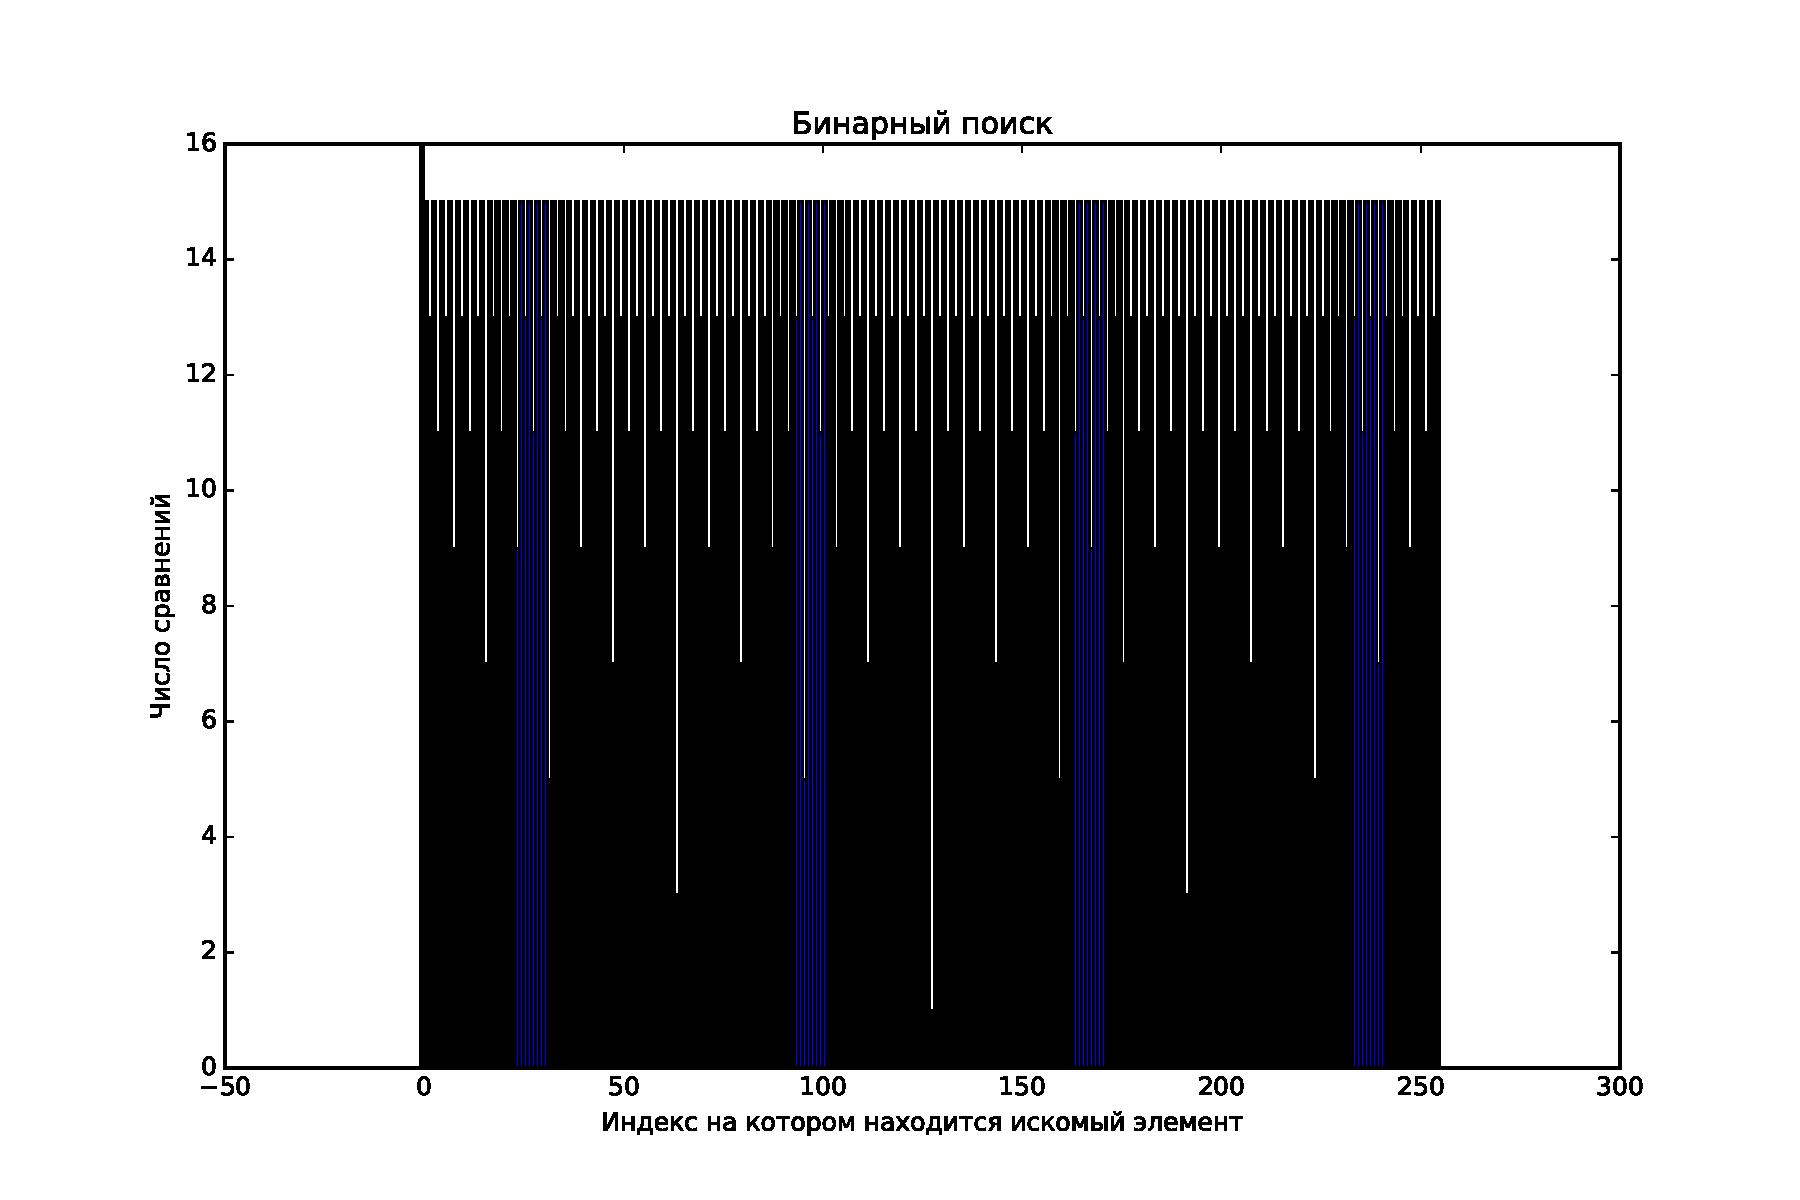
\includegraphics[width=\textwidth]{binary.pdf}
	\caption{График зависимости числа сравнений от индекса элемента для бинарного поиска}
	\label{fig:bin_plot}
\end{figure}

Среднее число операций сравнения полученное при замерах для бинарного поиска равно 17. Для линейного поиска это число составляет 521.

\section{Вывод}

Алгоритм бинарного поиска превосходит линейный поиск по эффективности относительно числа производимых сравнений. Так для нахождения максимального элемента бинарный поиск производит 21 операцию сравнения, тогда как линейный поиск осуществляет для этого 1041 операцию. При это для нахождения минимального элемента бинарный поиск производит 19 операций,а линейный одну. В среднем же бинарный поиск выполняет меньше операций сравнения, чем линейный алгоритм.

Если в формулу~\ref{eq:lin_standart_case} подставить $k_1 = 0$ и $k_2 = 1$, т.~е. одна операция сравнения на каждой итерации цикла, теоретическое среднее число операций сравнения получается равным $1 + \frac{1041}{2} + \frac{1}{1042} \approx 521$, что совпадает со средним числом сравнений полученным на практике.

Максимальное число операций сравнения для бинарного поиска составляет 21. При этом количество просматриваемых элементов равно 11, что также соответствует теоретической оценке при подстановке $n = 1041$ в формулу~\ref{eq:bin_cnt_elems}: $\lfloor \log_2{1041} \rfloor + 1 = 10 + 1 = 11$.

Однако, бинарный поиск требует упорядоченности массива, что сужает допустимый спектр входных данных, тогда как линейный поиск таких требований не накладывает.


\clearpage